\documentclass{article}

\usepackage{amsmath}
\usepackage{amscd}
\usepackage[tableposition=top]{caption}
\usepackage{ifthen}
\usepackage[utf8]{inputenc}

\usepackage{Sweave}
\begin{document}

\title{Estimating HIV transmission rates with \texttt{rcolgem}}
\author{Erik M Volz}
\date{\today}
\maketitle

This vignette will demonstrate how to use a coalescent models as described in~\cite{volz2012complex} to estimate transmission rate parameters given a pathogen genealogy.

Suppose an epidemic occurs according to dependent susceptible-infected-recovered process, and a given infected individual generates a new infection at the rate $\beta S I$, where $S$ is the number susceptible and $\beta$ is the transmission rate.
%\begin{align}
%I \xrightarrow{\beta S I} 2I 
%\end{align}
Furthermore, infected individuals will be removed from the population at per capita rate $\gamma$. 
At a single point in time, a random sample of $n=75$ infected individuals is taken and the genealogy is reconstructed from the history of transmissions.
We have simulated such a dataset using MASTER 1.10\cite{vaughan2013stochastic}, which can be loaded by
\begin{Schunk}
\begin{Sinput}
> library(rcolgem)
> tree <- read.tree(system.file( 'extdata/sirModel0.nwk', package='rcolgem'))
\end{Sinput}
\end{Schunk}
And, the epidemic trajectory information can be loaded by
\begin{Schunk}
\begin{Sinput}
> library(rjson)
> epidata <- fromJSON(file=system.file('extdata/sirModel0.json', package='rcolgem')) 
\end{Sinput}
\end{Schunk}
The true parameter values are given in table~\ref{tab:parms}.
The file used to simulate the data can be viewed by \texttt{ file.show( system.file('extdata/sirModel0.xml', package=rcolgem)) }. 

%Let's plot the epidemic trajectory along with the time of sampling ($t=12$):
%<<>>=
%plot( epidata$t, epidata$I , type='line')
%abline( v = 12, col='red') 
%@

We will fit a simple ODE model to the genealogy:
\begin{align}
\dot{S} &= -\beta S I  \\
\dot{I} &= \beta S I - \gamma I
\end{align}
Relevant parameters of the system are the transmission rate $\beta$, recovery rate $\gamma$, initial population size $S(0)$ and initial number infected $I(0)$. 
Not all parameters are identifiable from these data, so we will assume prior knowledge of $S(0)$ and $\gamma$ and focus on estimating $\beta$ and the nuisance parameter $I(0)$. Note that an imprecise estimate of $S(0)$ is also possible. 



\begin{table}
\caption{ Parameter symbols and values. \label{tab:parms} }
\begin{center}
	\begin{tabular}{lll}
		\hline 
		Parameter & Symbol & Value \\
		\hline
		Duration infection & $1/\gamma$ & 1  \\
		Transmission rate & $\beta$ & 2.0002e-4 \\
		Population size  & $S(0)$ & 9999 \\
		Initial num infected & $I(0)$ & 1 \\
		Time of sampling & $T$ & 12 \\
		\hline 
	\end{tabular}
\end{center}
\end{table}

Create a list to store the true parameter values:
\begin{Schunk}
\begin{Sinput}
> parms_truth <- list( beta = .00020002, gamma = 1, S0 = 9999, t0 = 0 )
\end{Sinput}
\end{Schunk}
Note that the true value of $R_0$ is $\beta S(0) / \gamma = 2$. 

And, create a tree with dated tips and internal nodes: 
\begin{Schunk}
\begin{Sinput}
> sampleTimes <- rep(12, 75)
> names(sampleTimes) <- tree$tip.label
> bdt <- binaryDatedTree( tree, sampleTimes=sampleTimes) 
\end{Sinput}
\end{Schunk}
Note that the vector of sample times must have names corresponding to the taxon labels in tree. 




In order to fit this model, we need to express the equations in a canonical format:
\begin{Schunk}
\begin{Sinput}
> births <- c( I = 'parms$beta * S * I' )
> deaths <- c( I = 'parms$gamma * I' )
> nonDemeDynamics <- c(S = '-parms$beta * S * I')
\end{Sinput}
\end{Schunk}
The \texttt{births} vector gives the total rate that all infected generate new infections and \texttt{deaths} gives the rate that lineages are terminated. 
The \texttt{nonDemeDynamics} vector gives the equations for state variables that aren't directly involved in the genealogy (e.g. because a pathogen never occupies a susceptible host by definition). 

Each element of the vectors is a string that will be parsed as R code and evaluated, so it is important to write it exactly as you would if you were solving the equations in R.
Also note that the object \texttt{parms} is accessible to these equations, which is a list of parameters- this may include parameters to be estimated.
Also note that we \emph{must} give names to the vectors, and these names must correspond to the names of the demes. 

We will use these initial conditions
\begin{Schunk}
\begin{Sinput}
> x0 <- c(I=1, S= unname(parms_truth$S0) )
> t0 <- bdt$maxSampleTime - max(bdt$heights) -1 
\end{Sinput}
\end{Schunk}
The time of origin $t_0$ is chosen somewhat arbitrarily, but should occur before the root of the tree. 

Now we can calculate the likelihood of the tree and assess how long it takes:
\begin{Schunk}
\begin{Sinput}
> print( 
+ system.time( 
+ print(
+   coalescent.log.likelihood(
+     bdt
+     , births, deaths, nonDemeDynamics
+     , t0, x0
+     , parms=parms_truth
+     , fgyResolution = 1000
+     , integrationMethod = 'rk4')
+ )))
\end{Sinput}
\begin{Soutput}
[1] 67.75564
   user  system elapsed 
  0.668   0.000   0.668 
\end{Soutput}
\end{Schunk}
Note that changing the \texttt{integrationMethod} (choose `euler'), \texttt{censorAtHeight} (only fit to part of the tree) and \texttt{fgyResolution} (set to a smaller value) options can dramatically speed up the calculation at the cost of some accuracy. 

We can fit the model using maximum likelihood with the \texttt{bbmle} or \texttt{stats4} packages. 
\begin{Schunk}
\begin{Sinput}
> 	library(bbmle)
\end{Sinput}
\end{Schunk}
First, create the objective function to be minimized:
\begin{Schunk}
\begin{Sinput}
> obj_fun <- function(lnbeta, lnI0)
+ {
+ 	beta <- exp(lnbeta)
+ 	I0 <- exp(lnI0)
+ 	parms <- parms_truth
+ 	parms$beta <- beta
+ 	x0 <- c(I=unname(I0), S = unname(parms$S0) )
+ 	mll <- -coalescent.log.likelihood(
+ 		bdt
+ 		, births, deaths, nonDemeDynamics
+ 		,  t0, x0
+ 		, parms=parms
+ 		, fgyResolution = 1000
+ 		, integrationMethod = 'rk4')
+ 	print(paste(mll, beta, I0))
+ 	mll
+ }
\end{Sinput}
\end{Schunk}
Note that this uses log-transformation for variables that must be positive (like rates and population sizes).

We can then fit the model by running
\begin{Schunk}
\begin{Sinput}
> fit <- mle2(
+   obj_fun
+   , start=list(lnbeta=log(parms_truth$beta*.75), lnI0=log(1))
+   , method='Nelder-Mead'
+   , optimizer='optim' 
+   , control=list(trace=6, reltol=1e-8)
+ )
\end{Sinput}
\end{Schunk}
Note that we are starting the optimizer far from the true parameter values.
If fitting a model to real data, it is recommended to try many different starting conditions over a large range of values.  
The optimizer would take a few minutes to run, so instead we will load the results:
\begin{Schunk}
\begin{Sinput}
> 	load( system.file('extdata/sirModel0-fit.RData', package='rcolgem') )
> 	AIC(fit)
\end{Sinput}
\begin{Soutput}
[1] -145.7974
\end{Soutput}
\begin{Sinput}
> 	logLik(fit)
\end{Sinput}
\begin{Soutput}
'log Lik.' 74.89871 (df=2)
\end{Soutput}
\begin{Sinput}
> 	coef(fit)
\end{Sinput}
\begin{Soutput}
    lnbeta       lnI0 
-8.4748155  0.1351695 
\end{Soutput}
\begin{Sinput}
> 	exp(coef(fit))
\end{Sinput}
\begin{Soutput}
      lnbeta         lnI0 
0.0002086577 1.1447308446 
\end{Soutput}
\begin{Sinput}
> 	# how biased is the estimate? 
> 	exp(coef(fit)['lnbeta']) - parms_truth$beta
\end{Sinput}
\begin{Soutput}
      lnbeta 
8.637689e-06 
\end{Soutput}
\end{Schunk}

We can compare the fitted model to the true number of infected through time, which is shown in figure~\ref{fig:results0}.
\begin{Schunk}
\begin{Sinput}
> beta <- exp(coef(fit)['lnbeta'])
> I0 <- exp(coef(fit)['lnI0'])
> parms <- parms_truth
> parms$beta <- beta
> x0 <- c(I=unname(I0), S = unname(parms$S0) )
> o <- solve.model.unstructured(t0, x0, births,  deaths
+   , nonDemeDynamics, parms)
> otruth <- solve.model.unstructured(t0, x0, births,  deaths
+   , nonDemeDynamics, parms_truth)
> plot(epidata$t, epidata$I, type='line'
+   , ylim=c(0, 100+max(max(o[,2]),max(epidata$I))))
> lines(o[,1], o[,2], col='red' )
> lines(otruth[,1], otruth[,2], col='blue' )
\end{Sinput}
\end{Schunk}
\begin{figure}
	\begin{center}
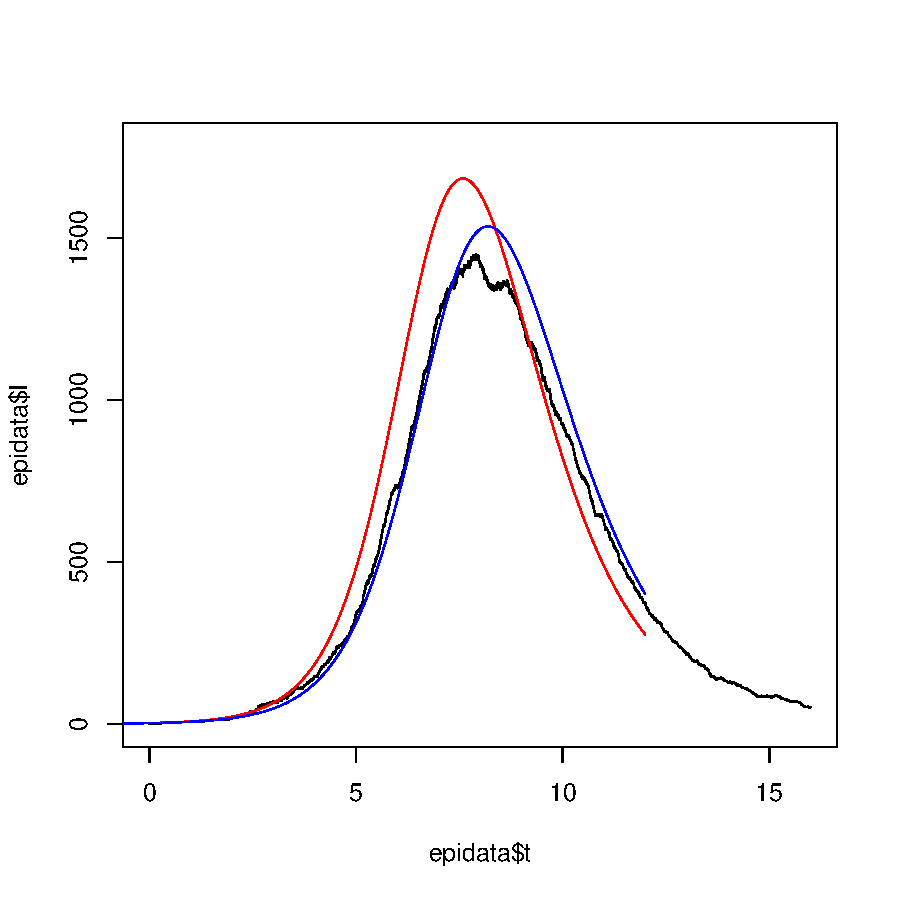
\includegraphics{sir_vignette-results0}
	\end{center}
	\caption{The actual (black) and estimated (red) number of infections through time. The blue line shows the SIR model prediction under the true parameter values.  \label{fig:results0} }
\end{figure}


We can calculate a confidence interval for the transmission rate using likelihood profiles:
\begin{Schunk}
\begin{Sinput}
> profbeta <- profile(fit, which=1, alpha=.05
+   , std.err=1, trace=TRUE, tol.newmin=1 )
\end{Sinput}
\end{Schunk}
This takes a few minutes, so we will load the results:
\begin{Schunk}
\begin{Sinput}
> load( system.file('extdata/sirModel0-profbeta.RData',  package='rcolgem') )
\end{Sinput}
\end{Schunk}
We see that the confidence interval covers the true value:
\begin{Schunk}
\begin{Sinput}
> c( exp( confint( profbeta ) ), TrueVal=parms_truth$beta )
\end{Sinput}
\begin{Soutput}
       2.5 %       97.5 %      TrueVal 
0.0001901721 0.0002282366 0.0002000200 
\end{Soutput}
\end{Schunk}
And, we can visualize the profile (Figure~\ref{fig:profile}). 
\begin{Schunk}
\begin{Sinput}
> plot(profbeta)
> abline( v = log( parms_truth$beta) , col='red')
\end{Sinput}
\end{Schunk}
\begin{figure}
\begin{center}
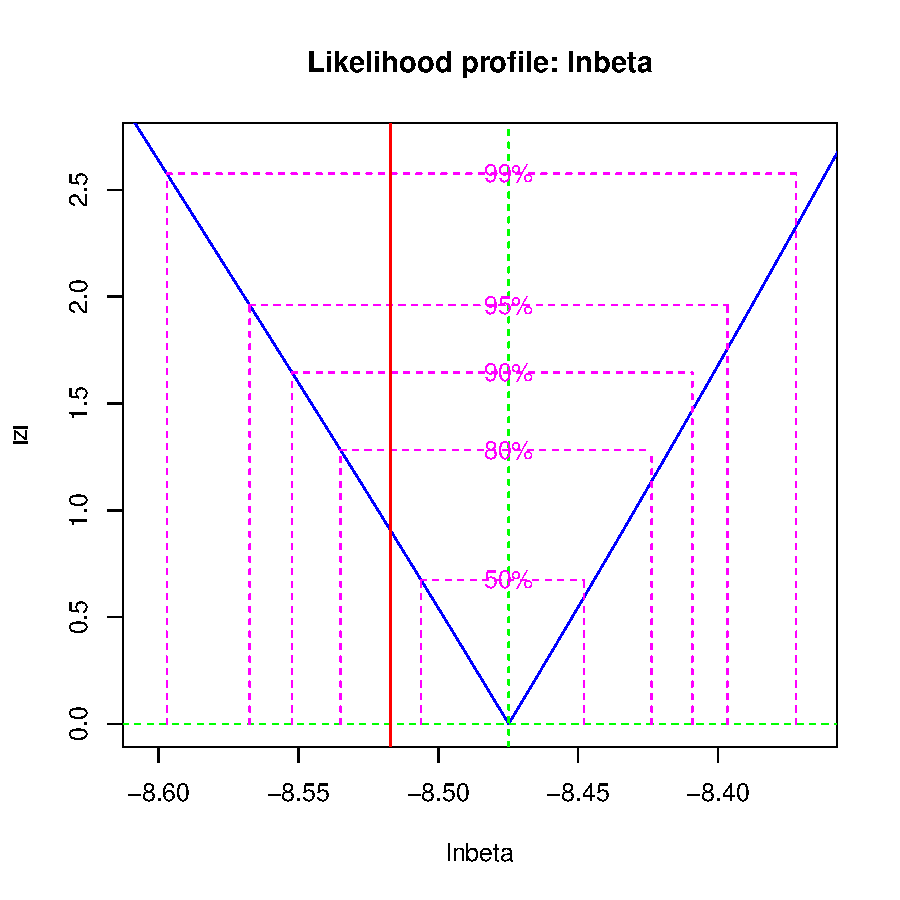
\includegraphics{sir_vignette-proffigure}
\end{center}
\caption{Likelihood profile for the transmission rate $\beta$ with confidence levels. The true parameter value is indicated by the vertical red line.\label{fig:profile}}
\end{figure}

\bibliographystyle{plain}
\bibliography{sir_vignette}
\end{document}


